%%==================================================
%% thanks.tex for SJTU Master Thesis
%% based on CASthesis
%% modified by wei.jianwen@gmail.com
%% version: 0.3a
%% Encoding: UTF-8
%% last update: Dec 5th, 2010
%%==================================================

\begin{thanks}
\iffalse
感谢Donald Knuth!

感谢Leslie Lamport!

感谢\LaTeX!

感谢ex!

感谢导师!

感谢NJU!

感谢父母!

感谢上帝!
\fi
%\iffalse
来到闵行这地方纯粹是个意外。三年前从未想过,当初一个不起眼的无奈选择竟会给己生带来如此大的偏差。

多少个夜晚,一个人走在东区回D29的路上,四周寂静无人,死气沉沉,陪伴我的只有内心的彷徨和苦闷。我到底做错了什么?为何要被生活如此捉弄?于是乎,不禁回想起大四在鼓楼校区的那段时光。傍晚时分陪你去安中楼,走在北园的梧桐道上,天空飘着细雨,地上铺就黄叶,旁边都是划满沧桑的建筑,北园秋天给我们的感觉如此安详美好。时光啊时光,请你再慢一些,让我可以牵着你走向更远。初中时候受某只影响,觉得筠子的《立秋》这首歌很好听很有feeling,便不知不觉于四季之中最欣赏秋天。此情此景想来是此生难再,当然,人的心境也已大有不同了。:)

痛苦过后是麻木,我尝试着用阿Q精神去麻醉自己,也开始朝向毕业大计努力。路是自己选择的,无论如何也要坚持走下去。这年5月确定了实习去处,6月投出了小论文,自己稍微心安了一些。在网易实习的那两个月,算是前两年中自己心无重担最愉悦闲适的一段时光,不仅是因为杭州的好山好水,更重要的是我可以暂时逃离闵行逃离西南某高校。自杭州回来后,照例开启了求职模式,还算幸运,自己期望的offer基本都拿到了。10月底与你在莘庄重逢,在翌日去帝都的火车上我意识到自己始终未能将你放下,虽然前途未卜,却仍然要感谢你能理解我这三年中的所作所为。

要致谢的还有很多。首先是我的父母,家庭是永久的栖息港湾,感谢他们二十余载不辞辛劳的抚育之恩,无论是在经济上还是精神上。接着是我的导师陈海波教授和老大臧斌宇教授,感谢他们在我读研期间给予的科研指导,以及在论文发表上提供的帮助,让我可以顺利毕业。还要感谢我的母校南京大学,``诚''、``朴''二字已深谙吾心,很庆幸能在钟灵毓秀的南京度过四年本科生活,让我可以自由汲取知识,并结识到一帮善解人意、积极向上的人生益友。launch、abo、lu007heng、msh、coboy、quicksort等等,感谢你们在最低谷最黑暗的岁月中给予我的鼓励支持。当然,最后还要感谢IPADS实验室的一众小伙伴们,尤其是翔哥和P哥,预祝今后在百度合作愉快。

自己一直向往自由随性的生活,能研究感兴趣的领域,能对一个人倾注感情,足矣!平心而论,这两年多的读研生活实在是和自己格格不入。世间没有后悔药,我能做到的只是不断让自己变得更强大。我不畏惧困难挫折,但奋斗过后我必定会反省自身,你究竟得到了什么?这段努力到底值不值得?

就把自己这在西南某高校两年多的经历当作生命中一段灰暗的小插曲吧。我遵守了三年前的那份承诺,你可以么?

\begin{figure}[!htbp]
  \centering
  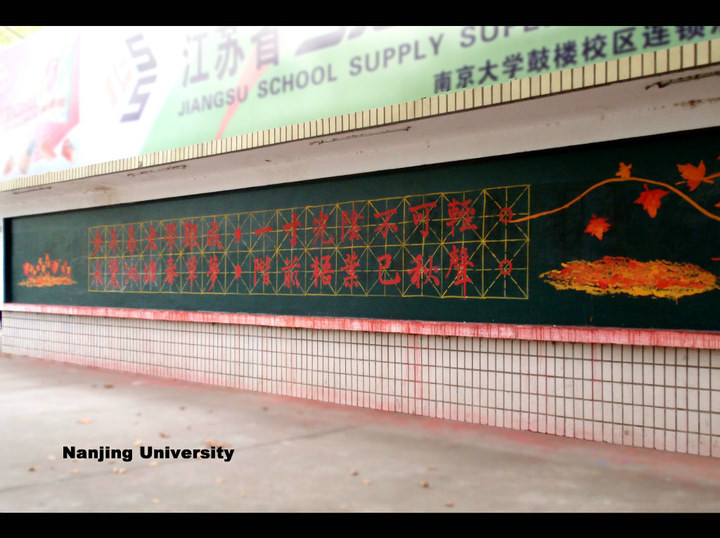
\includegraphics[width=0.7\textwidth]{ack/nju.jpg}
  %\bicaption[fig:nested]{嵌套式虚拟化示意}{嵌套式虚拟化示意}{Fig}{Illustration on Nested Virtualization}
\end{figure}
%\fi

\end{thanks}
